\chapter{FOBOS Hardware Configuration} \label{chap:hardware-config}
\section{Introduction}
FOBOS consists of Python scripts for acquisition and analysis and hardware for controller and DUT.
This chapter describes the harware setup and descibes preparing and programming the controller and DUT boards.
This chapter assumes familiarity with Xilinx ISE and Xilinx Imapct tools.

FOBOS hardware is composed of two boards and other devices. The first board is the Control Board which handles communication with the control PC, triggering the oscilloscope and clocking the DUT.
The other board is the DUT which hosts the DUT Wrapper and the DUT.
An oscilloscope captures the power traces and the control PC collects them for analysis. 
A power supply is used to power the DUT and a clock generator might be used to provide clock for the Control Board which provides it to the DUT.

\begin{center}

\begin{figure}
  \label{fig:fobos-capture}
  \caption{FOBOS Hardware}
  \centering
   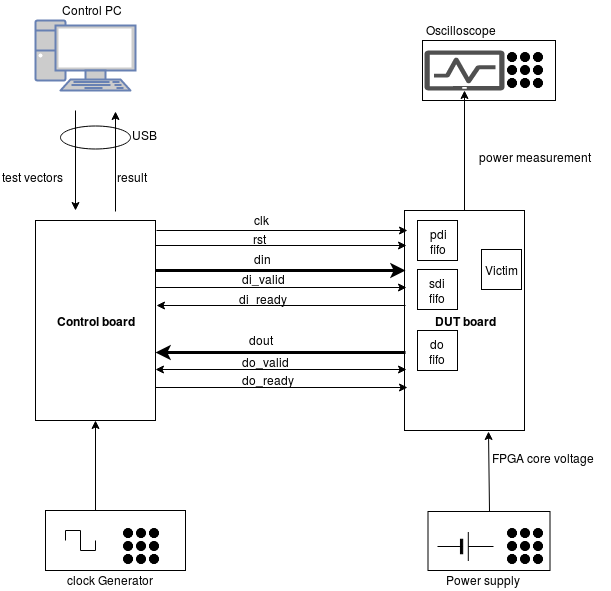
\includegraphics[scale=0.6]{../figures/FOBOS_Capture}
\end{figure}
\end{center}

\section{Hardware List}
\begin{enumerate}
  \item The control board (A standard FPGA board)
  \item The DUT board (A standard FPGA board)
  \item An oscilloscope (Agilent Technologies DSO6054A) 
  \item DC Power supply (Agilent E3620A)
  \item Clock generator (Instek SFG-2120 20 MHz)
  \item Control PC (A standard PC running Linux)
  \item Current probe (1mV/mA Tektronics CT-2 current sensing probe)
\end{enumerate}


\section{Programming the Control Board}

The source VHDL files for the controller are located at \texttt{fobos/source/vhdl}. You need to use Xilinx ISE to generate the bitstream file and use Xilinx Impact to load the bitstream
into the Control Board.

\subsection {Programming Steps}
\begin{enumerate}
  \item Create a new project using Xilinx ISE. In the New Project wizard, set the Project Settings per the control board used. 
  Make sure to select the values for Family, Device, Package and Speed (See Fig~\ref{fig:ctrl-design-properties} for an example).
  		\begin{figure} 
		\begin{center}
		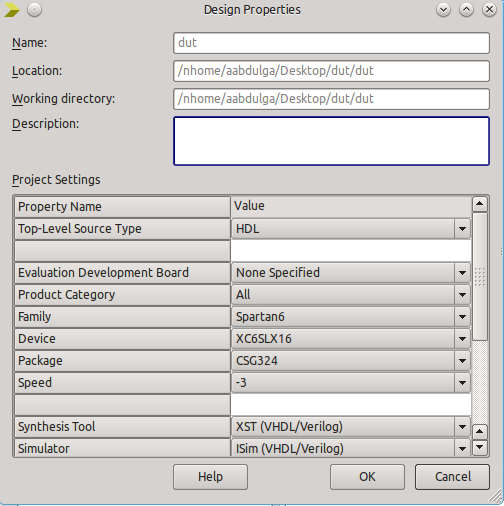
\includegraphics[scale=0.6]{figures/ctrl-design-properties}
		\caption{\label{fig:ctrl-design-properties}FOBOS Controller Desgin Properties}
		\end{center}
		\vspace{-1ex}
		\end{figure}
  \item From the Project menu, select Add Source... and add all files from \texttt{\$fobos/sources/common}.
  \item Repeat the previous step to add all vhdl files from \texttt{\$fobos/sources/vhdl/control}. Also, add the appropriate UCF file depending on the Control Board used (See Fig~\ref{fig:ctrl-add-sources}) .
		\begin{figure} 
		\begin{center}
		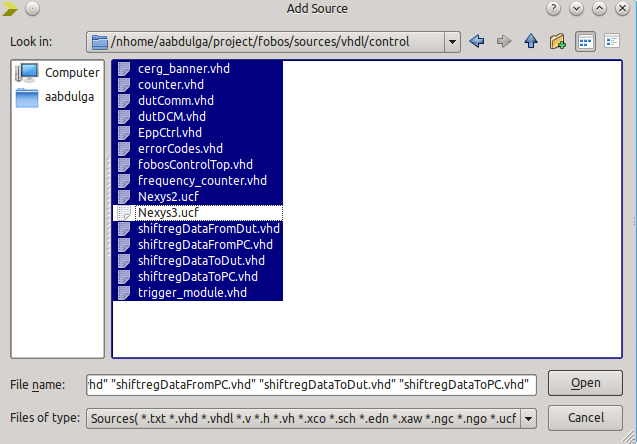
\includegraphics[scale=0.6]{figures/ctrl-add-sources}
		\caption{\label{fig:ctrl-add-sources}Adding Source Files to FOBOS Controller}
		\end{center} 
		\vspace{-1ex}
		\end{figure}
  \item Set the \texttt{fobosControlTopLevel} module as the top-level module for this project (See Fig~\ref{fig:ctrl-set-top-level}).
		\begin{figure} 
		\begin{center}
		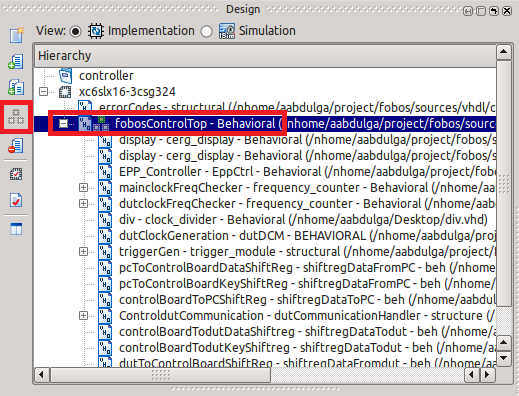
\includegraphics[scale=0.6]{figures/ctrl-set-top-level}
		\caption{\label{fig:ctrl-set-top-level}Setting Top-level Module}
		\end{center} 
		\vspace{-1ex}
		\end{figure}
  \item Generate the programming bit file for the control board by clicking "Generate Programming File" in the Processes window.
  \item Program the control board using Xilinx Impact. In the Processes window, click Configure Target Device (See Fig~\ref{fig:ctrl-run-impact}).
		\begin{figure} 
		\begin{center}
		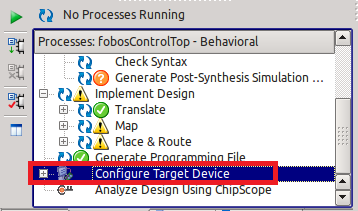
\includegraphics[scale=0.6]{figures/ctrl-run-impact}
		\caption{\label{fig:ctrl-run-impact}}
		\end{center}
		\vspace{-1ex}
		\end{figure}
  \item In the Impact window, click "Boundary Scan" then form the File menu, click "Initialize Chain" and assign the bit file to the FPGA. Now you may right-click the FPGA and click "Program".
		\begin{figure} 
		\begin{center}
		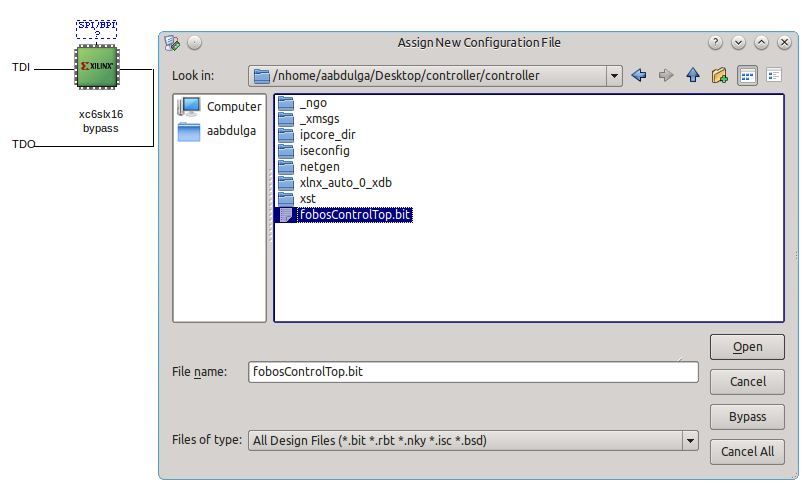
\includegraphics[scale=0.6]{figures/ctrl-program}
		\caption{\label{fig:ctrl-program}Progrmamming the Control Board}
		\end{center}
		\vspace{-1ex}
		\end{figure}
  \end{enumerate}

\section{DUT Board Programming}
The DUT board hosts two components:
\begin{enumerate}
 \item The DUT Wrapper : handles communication with the Control Board.
 \item The DUT (Victim) : the Device-Under-Test is user provided. This section assumes that this component is developed, instantiated and tested. Please see Chapter~\ref{chap:dut-dev} for more details.
\end{enumerate}

\subsection {Programming Steps}
\begin{enumerate}
  \item Create a new project using Xilinx ISE. In the New Project wizard set the Project Settings per the DUT Board used. 
  Make sure to select the values for Family, Device, Package and Speed (See Fig~\ref{fig:dut-design-properties} for an example).
		\begin{figure} 
		\begin{center}
		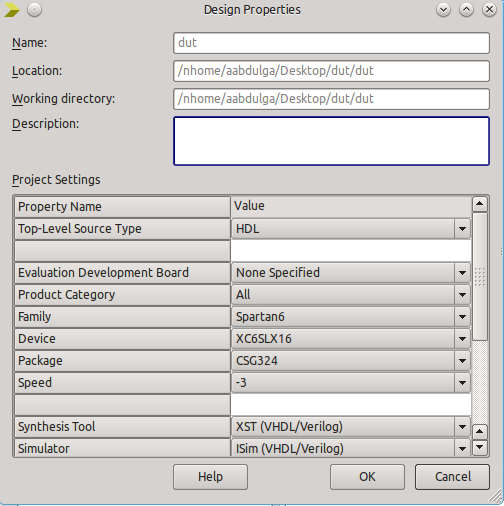
\includegraphics[scale=0.6]{figures/dut-design-properties}
		\caption{\label{fig:dut-design-properties}DUT Design Properties}
		\end{center}
		\vspace{-1ex}
		\end{figure}
  \item From the Project menu select Add Source... and add all files from \texttt{\$fobos/sources/common}.
  \item Repeat the previous process to add all vhdl files from \texttt{\$fobos/sources/vhdl/DUT} and make sure to add the appropriate UCF file depending on the DUT board used (See Fig~\ref{fig:dut-add-sources}).
  	\item Add the DUT (victim) vhdl files to the project (user provided).
		\begin{figure} 
		\begin{center}
		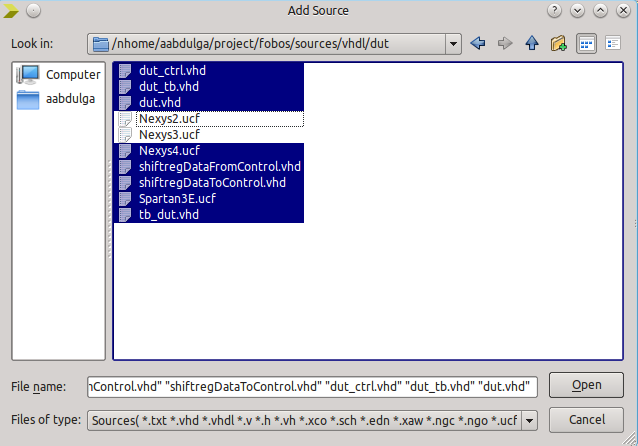
\includegraphics[scale=0.6]{figures/dut-add-sources}
		\caption{\label{fig:dut-add-sources}DUT Add Sources}
		\end{center}
		\vspace{-1ex}
		\end{figure}
  \item (Optional) You may choose to avoid using block RAMs in the implementation since this may affect attack difficulty.
     \begin{enumerate}
	\item Make sure to select the "Implementation" view.
        \item Right-click the Synthesize-XST process.
	\item In the Preocess Properties window, select HDL Options and select "Distributed" for the RAM Style property (See Fig~\ref{fig:dut-ram-style}).
	\item Click OK.
		\begin{figure} 
		\begin{center}
		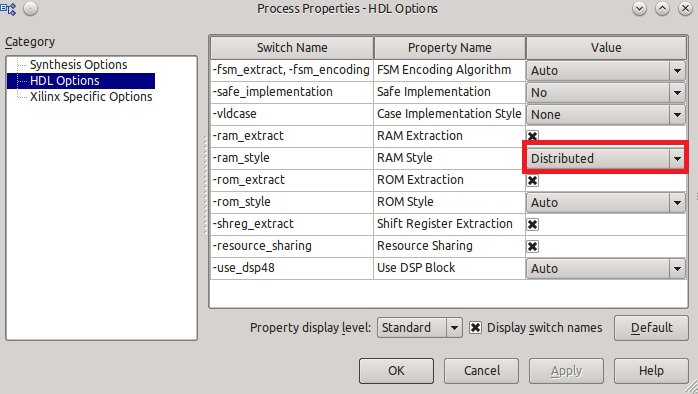
\includegraphics[scale=0.6]{figures/dut-ram-style}
		\caption{\label{fig:dut-ram-style}DUT RAM Style}
		\end{center}
		\vspace{-3ex}
		\end{figure}
     \end{enumerate}
  \item Set \texttt{FOBOS\_DUT} as the top-level module in this project.
		\begin{figure} 
		\begin{center}
		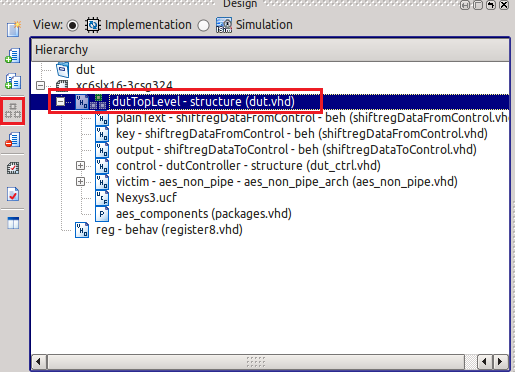
\includegraphics[scale=0.6]{figures/dut-set-top-level}
		\caption{\label{fig:dut-set-top-level}Set DUT Top-level}
		\end{center}
		\vspace{-3ex}
		\end{figure}
  \item Generate the programming bit file for the DUT by clicking "Generate Programming File" in the Processes window.
  \item Program the DUT using Xilinx Impact. In the Processes window, click Configure Target Device (See Fig~\ref{fig:dut-run-impact}).
		\begin{figure} 
		\begin{center}
		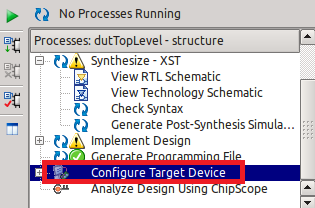
\includegraphics[scale=0.6]{figures/dut-run-impact}
		\caption{\label{fig:dut-run-impact}}
		\end{center}
		\vspace{-3ex}
		\end{figure}
  \item In the Impact window, click "Boundary Scan" then form the File menu, click "Initialize Chain" and assign the bit file to the FPGA. Now you may right-click the FPGA and click "Program".
		\begin{figure} 
		\begin{center}
		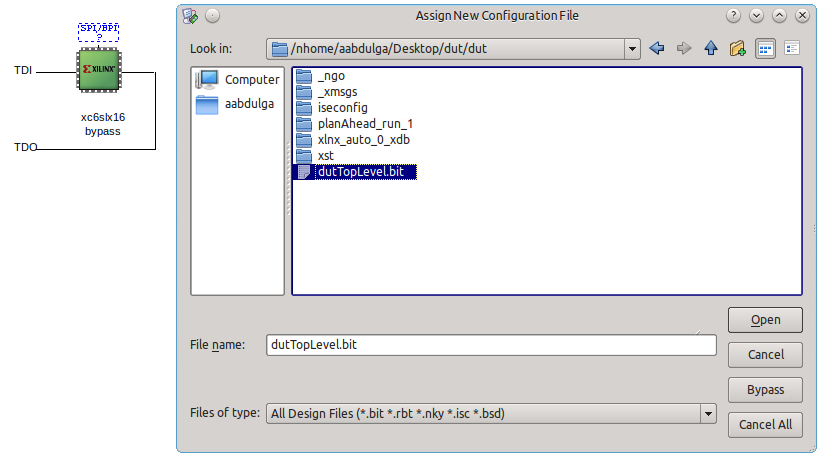
\includegraphics[scale=0.6]{figures/dut-program}
		\caption{\label{fig:dut-program}Progrmamming DUT}
		\end{center}
		\vspace{-3ex}
		\end{figure}
  \end{enumerate}


\section{Oscilloscope Configuration}
Ocsilloscope is connected to the PC via Ethernet. IP configuration must be completed on the oscilloscope for the PC to be able to collect traces. 
The oscillopscope used in current setup is Agilent DSO6054A. To configure IP on this oscilloscope, please refer to vendor's documentation.

\section{Connecting the Hardware}

To connect FOBOS hardware, follow these steps:
  \begin{enumerate}
  \item Connect control board to power and ground.
  \item Connect control board tirgger output the oscilloscope trigger channel.
  \item Connect the control board to the DUT (see details below).
  \item Connect the control board to the PC running FOBOS software using USB.
  \item Connect clock generator to control board. Set the clock generator to desired clock.
  \item Connect the current probe to the oscilloscope.
  \item Connect the current probe to the DUT's ground.
  \item Connect DUT to power making sure that the current probe is measuring the current.
  \item Connect DUT to power supply ground.
  \end{enumerate}
  
The following subsections ilustrate how to connect different FPGA boards as control and victim boards.

\subsection{Nexys3 Control Board - Nexys3 DUT}

This section describes connecting a Digilent Nexys3 Control board to a Nexys3 DUT board.
Nexys3 board includes a Xilinx Spartan6 FPGA. This board can use PMOD connectors for I/O.
It also descibes connections to other devices like the oscillopscope. For a high-level FOBOS hardware diagram, please refer to Figure~\ref{fig:fobos-capture}.

The two boards are connected using the PMOD port C and D. Some pins in port A and B are used to connect to the oscillopscope and the clock generator.
\newline
Note that the two boards must share GND. PMOD ports C and D are connected, each pin to its corresponding pin in the other board (e.g. JA1 $->$ JA1 and GND$->$ GND). 
However the 3.3 V pin is not connected in the PMOD connector.
\newline
\newline
\textbf{PMOD connector pin assignment on the control board}
\newline
\newline
\begin{array}{ | l | l | l | l | }
\hline
	PORT A & PORT B & PORT C & PORT D \\ \hline
	JA1: & JB1: EXTClock & JC1: DUTClock & JD1: reset \\ \hline
	JA2: & JB2: & JC2: do\_ready & JD2: di\_ready \\ \hline
	JA3: trigger  & JB3: & JC3: din(3) & JD3: dout(3) \\ \hline
	JA4: & JB4: & JC4: din(1) & JD4: dout(1) \\ \hline
	JA7: & JB7: & JC7: do\_valid & JD7: \\ \hline
	JA8: & JB8: & JC8: & JD8: di\_valid \\ \hline
	JA9: & JB9: & JC9: din(2) & JD9: dout(2) \\ \hline
	JA10: & JB10: & JC10: din(0) & JD10: dout(0) \\ \hline
\end{array}
\newline
\newline
\textbf{PMOD connector pin assignment on the DUT  board}
\newline
\newline
	\begin{array}{ | l | l | l | l | }
\hline
	PORT A & PORT B & PORT C & PORT D \\ \hline
	JA1: & JB1: & JC1: DUTClock & JD1: reset \\ \hline
	JA2: & JB2: & JC2: do\_ready & JD2: di\_ready \\ \hline
	JA3: & JB3: & JC3: din(3) & JD3: dout(3) \\ \hline
	JA4: & JB4: & JC4: din(1) & JD4: dout(1) \\ \hline
	JA7: & JB7: & JC7: do\_valid & JD7: \\ \hline
	JA8: & JB8: & JC8: & JD8: di\_valid \\ \hline
	JA9: & JB9: & JC9: din(2) & JD9: dout(2) \\ \hline
	JA10: & JB10: & JC10: din(0) & JD10: dout(0) \\ \hline
\end{array}


\newline
